% Quantitative panel generated from archived E02 data; provenance in calculations.
\begin{minipage}{0.96\linewidth}
\centering
\begin{tikzpicture}[r/.style={draw,rounded corners=2pt,text width=30mm,align=center,font=\small,minimum height=14mm}]
\node[r] (a) at (0,0) {形式验证\\依规格与检查器};
\node[r] (b) at (3.7,0) {执行反馈\\依覆盖与环境};
\node[r] (c) at (7.4,0) {学习式评审\\依模型与输入};
\node[r] (d) at (11.1,0) {内在信号\\依代理的有效性};
\draw[->] (a)--(b);\draw[->] (b)--(c);\draw[->] (c)--(d);
\end{tikzpicture}

\vspace{3mm}
{\small 上：文献的定性层级，不是测量定律。下：E02 的已实现方案，不能与上方逐格对应。}
\vspace{2mm}

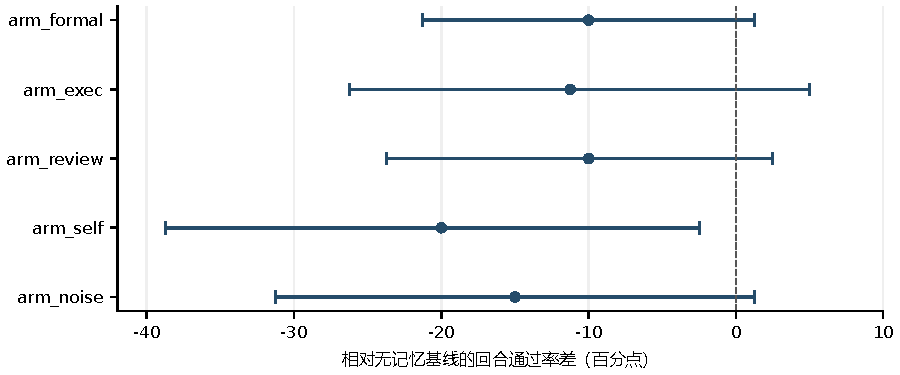
\includegraphics[width=\linewidth]{figures/generated/ch04-e02-effects.pdf}
\end{minipage}
